\documentclass[12pt,compress,english,utf8,t,usenames,dvipsnames]{beamer}
\usepackage[ngerman, english]{babel}


\title{Hierarchical Temporal Memory}
% \subtitle{And The Theory of Thousand Brains Intelligence}
\subtitle{A Theoretical Framework for the Neocortex}
\author{Felix Karg}


\graphicspath{ {../template/} {./graphics/} {../template_tex/} } % add further graphics paths here



\usepackage{etex}
\usepackage{graphicx}
\usepackage[export]{adjustbox}
\usepackage{multicol}
\usepackage{pdfpcnotes}
\usepackage{pdfpages}
% \usepackage[dvipsnames]{xcolor}


% \usepackage{minted}
% \usemintedstyle{pastie}


\usetheme[numbering=fraction, progressbar=frametitle]{metropolis}


\date{December 29, 2020}
% \date{12. Juli 2019}


% \institute{Add Your Institute here}
% \titlegraphic{\vspace{4cm} \hspace{7cm} \includegraphics[height=2cm]{Logo_INST}}
% \titlegraphic{\vspace{4cm} \hspace{7cm} \Huge\LaTeX}

\iftwocols
\AtBeginSection[]
{
    \large
    \begin{frame}{Agenda}
        \begin{multicols}{2}
            \tableofcontents[currentsection]
        \end{multicols}
        \clearpage
    \end{frame}
}

\AtBeginSubsection[]
{
    \large
    \begin{frame}{Agenda}
        \begin{multicols}{2}
            \tableofcontents[currentsection,currentsubsection]
        \end{multicols}
        \clearpage
    \end{frame}
}

\else

\AtBeginSection[]
{
    \large
    \begin{frame}{Agenda}
        \tableofcontents[currentsection]
        \clearpage
    \end{frame}
}

\AtBeginSubsection[]
{
    \large
    \begin{frame}{Agenda}
        \tableofcontents[currentsection,currentsubsection]
        \clearpage
    \end{frame}
}
\fi


\begin{document}

\maketitle

% multicols from:
% https://tex.stackexchange.com/questions/24343/splitting-toc-into-two-columns-on-single-frame-in-beamer

%%%%%%%%%%%%%%%%%%%%%%%%%%%%%%%%%%%%%%%%%%%%%%%%%%%%%%%%%%%%%%%%%%%%%%%%%%%%%%%%%%%%%%%%%%%%%%%%%%%%%%%%%%%%%%%%%%%

\iftwocols
\begin{frame}{Agenda}
    \large
    \begin{multicols}{2}
%        \tableofcontents[hidesubsections]
        \tableofcontents[]
    \end{multicols}
    % \clearpage
\end{frame}

\else

\begin{frame}{Agenda}
    \large
%   \tableofcontents[hidesubsections]
    \tableofcontents[]
    % \clearpage
\end{frame}
\fi


\newcommand{\code}[1]{
    \begin{center}
    \setlength{\fboxrule}{1pt}
    \setlength{\fboxsep}{8pt}
        {\fbox{\parbox{0.81\textwidth}{#1}}}
   \end{center}
}

\newenvironment{codeboxed}[1]
        {\begin{minipage}{\linewidth}\begin{center}#1\\[1ex]\begin{tabular}{|p{\textwidth}|}\hline}
        {\\\hline\end{tabular}\end{center}\end{minipage}}


\newcommand{\backupbegin}{
   \newcounter{finalframe}
   \setcounter{finalframe}{\value{framenumber}}
}

\newcommand{\backupend}{
   \setcounter{framenumber}{\value{finalframe}}
}


\newcommand{\mailto}[1]{
    \href{mailto:#1}{#1}
}

\newcommand{\todo}[1]{
    {\Large\color{red}{(TODO: #1)}}
}

% \definecolor{green1}{RGB}{38, 69, 37} % #264525
\definecolor{green1}{RGB}{72, 129, 69} % #488145
% \definecolor{blue1}{RGB}{7, 43, 94} % #072b5e
\definecolor{blue1}{RGB}{14, 82, 179} % #0e52b3
% \definecolor{violet1}{RGB}{58, 38, 68} % #3a2644
\definecolor{violet1}{RGB}{108, 72, 126} % #6c487e
% \definecolor{orang1}{RGB}{, , 0} % #663400
\definecolor{orang1}{RGB}{193, 98, 0} % #c16200


\newcommand{\green}[1]{
    \textcolor{green1}{#1}
}
\newcommand{\blue}[1]{
    \textcolor{blue1}{#1}
}
\newcommand{\vio}[1]{
    \textcolor{violet1}{#1}
}
\newcommand{\orang}[1]{
    \textcolor{orang1}{#1}
}

% 
\usepackage{etex}
\usepackage{graphicx}
\usepackage[export]{adjustbox}
\usepackage{multicol}
\usepackage{pdfpcnotes}
\usepackage{pdfpages}
% \usepackage[dvipsnames]{xcolor}


% \usepackage{minted}
% \usemintedstyle{pastie}


\usetheme[numbering=fraction, progressbar=frametitle]{metropolis}


\date{December 29, 2020}
% \date{12. Juli 2019}


% \institute{Add Your Institute here}
% \titlegraphic{\vspace{4cm} \hspace{7cm} \includegraphics[height=2cm]{Logo_INST}}
% \titlegraphic{\vspace{4cm} \hspace{7cm} \Huge\LaTeX}

\iftwocols
\AtBeginSection[]
{
    \large
    \begin{frame}{Agenda}
        \begin{multicols}{2}
            \tableofcontents[currentsection]
        \end{multicols}
        \clearpage
    \end{frame}
}

\AtBeginSubsection[]
{
    \large
    \begin{frame}{Agenda}
        \begin{multicols}{2}
            \tableofcontents[currentsection,currentsubsection]
        \end{multicols}
        \clearpage
    \end{frame}
}

\else

\AtBeginSection[]
{
    \large
    \begin{frame}{Agenda}
        \tableofcontents[currentsection]
        \clearpage
    \end{frame}
}

\AtBeginSubsection[]
{
    \large
    \begin{frame}{Agenda}
        \tableofcontents[currentsection,currentsubsection]
        \clearpage
    \end{frame}
}
\fi


\begin{document}

\maketitle

% multicols from:
% https://tex.stackexchange.com/questions/24343/splitting-toc-into-two-columns-on-single-frame-in-beamer

%%%%%%%%%%%%%%%%%%%%%%%%%%%%%%%%%%%%%%%%%%%%%%%%%%%%%%%%%%%%%%%%%%%%%%%%%%%%%%%%%%%%%%%%%%%%%%%%%%%%%%%%%%%%%%%%%%%

\iftwocols
\begin{frame}{Agenda}
    \large
    \begin{multicols}{2}
%        \tableofcontents[hidesubsections]
        \tableofcontents[]
    \end{multicols}
    % \clearpage
\end{frame}

\else

\begin{frame}{Agenda}
    \large
%   \tableofcontents[hidesubsections]
    \tableofcontents[]
    % \clearpage
\end{frame}
\fi


\newcommand{\code}[1]{
    \begin{center}
    \setlength{\fboxrule}{1pt}
    \setlength{\fboxsep}{8pt}
        {\fbox{\parbox{0.81\textwidth}{#1}}}
   \end{center}
}

\newenvironment{codeboxed}[1]
        {\begin{minipage}{\linewidth}\begin{center}#1\\[1ex]\begin{tabular}{|p{\textwidth}|}\hline}
        {\\\hline\end{tabular}\end{center}\end{minipage}}


\newcommand{\backupbegin}{
   \newcounter{finalframe}
   \setcounter{finalframe}{\value{framenumber}}
}

\newcommand{\backupend}{
   \setcounter{framenumber}{\value{finalframe}}
}


\newcommand{\mailto}[1]{
    \href{mailto:#1}{#1}
}

\newcommand{\todo}[1]{
    {\Large\color{red}{(TODO: #1)}}
}

% \definecolor{green1}{RGB}{38, 69, 37} % #264525
\definecolor{green1}{RGB}{72, 129, 69} % #488145
% \definecolor{blue1}{RGB}{7, 43, 94} % #072b5e
\definecolor{blue1}{RGB}{14, 82, 179} % #0e52b3
% \definecolor{violet1}{RGB}{58, 38, 68} % #3a2644
\definecolor{violet1}{RGB}{108, 72, 126} % #6c487e
% \definecolor{orang1}{RGB}{, , 0} % #663400
\definecolor{orang1}{RGB}{193, 98, 0} % #c16200


\newcommand{\green}[1]{
    \textcolor{green1}{#1}
}
\newcommand{\blue}[1]{
    \textcolor{blue1}{#1}
}
\newcommand{\vio}[1]{
    \textcolor{violet1}{#1}
}
\newcommand{\orang}[1]{
    \textcolor{orang1}{#1}
}




\newif\ifonline
\onlinefalse
% \onlinefalse


%%%%%%%%%%%%%%%%%%%%%%%%%%%%%%%%%%%%%%%%%%%%%%%%%%BEGINNING%%%%%%%%%%%%%%%%%%%%%%%%%%%%%%%%%%%%%%%%
% \section{Examples}

\begin{frame}[c]
     Here a citation: \cite{benchcpp}
\end{frame}

\begin{frame}[c]{Example slide}
    \Large
    \begin{itemize}[<+->]
        \item First Element
        \item Second Element
        \item Third Element
    \end{itemize}
\end{frame}

\begin{frame}[c]{Other example slide}
    \Large
    \begin{itemize}[<+(1)->]
        \item First Element
        \item Second Element
        \item Third Element
    \end{itemize}
\end{frame}

\begin{frame}[c]{Yet another example slide}
    \Large
    \begin{itemize}
        \item First Element
            \pause
        \item Second Element
            \pause
        \item Third Element
    \end{itemize}
\end{frame}








\section{Conclusion}




\section{Core Concepts}
\section{Overview}


\begin{frame}[c]{What is HTM?}
    \begin{itemize}[<+(1)->]
        \item biologically constrained \textbf{theory of intelligence}
        \item originally described in ''On Intelligence''
        \item \textbf{based on neuroscience} of the brain
    \end{itemize}

    \vspace{0.5cm}

    \pause

    $\rightarrow$ Learning Algorithms \pause (of the brain)
\end{frame}


\begin{frame}[c]{Attributes of HTM Algorithms}
    \begin{itemize}[<+(1)->]
        \item can store, learn, infer and recall higher-order sequences
        \item learns unsupervised time-based patterns in unlabeled data on continuous streams
        \item robust against noise
        \item can learn multiple patterns at once
        \item suited for prediction, anomaly detection, classification
        \item tested and implemented in software
        \item commercially used
    \end{itemize}
\end{frame}





\subsection{Hierarchy}


\begin{frame}[c]{Why Hierarchy?}
    \Large
    \pause
    If there is a connection cost, hierarchies are more efficient \cite{mengistu2016evolutionary}. 
    
    \pause
    Especially when tasks change regularly.
\end{frame}


\begin{frame}[c]{Why Hierarchy? II}
    \Large
    \begin{itemize}[<+(1)->]
        \item Reduced Training Time
        \item Reduced Memory Usage
        \item Introduce Generalizations
        \item Learned patterns are recombined at higher levels
        \item Transfer Learning
    \end{itemize}
\end{frame}


\begin{frame}[c]{What Hierarchy}
    \pause
                                        % trim = left bottom right top
    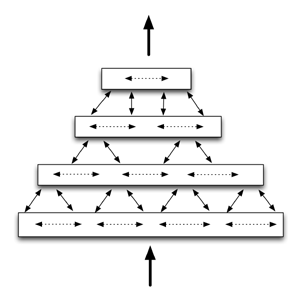
\includegraphics[width=\textwidth, trim = 0 55 0 60, clip]{hierarchy}
\end{frame}


\begin{frame}[c]{Example Application}
    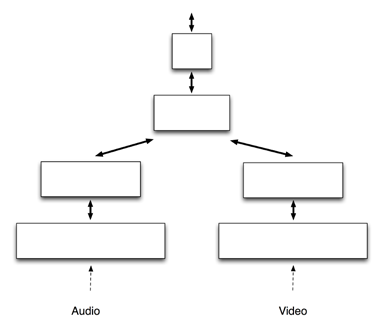
\includegraphics[height=0.9\textheight]{hierarchy_2} 
\end{frame}


\begin{frame}[c]{How Many Levels?}
    \Large
    \begin{itemize}[<+(1)->]
        \item They always learn the best representation
        \item Tradeoff between depth and layer size
        \item Simple problems can be solved with one region
    \end{itemize}
\end{frame}



\subsection{Regions}


\begin{frame}[c]{Region - Introduction}
    \pause
                                        % trim = left bottom right top
    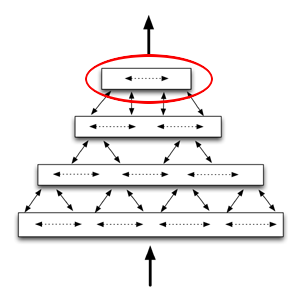
\includegraphics[width=\textwidth, trim = 0 55 0 54, clip]{region}
\end{frame}


\begin{frame}[c]{Region - Details}
    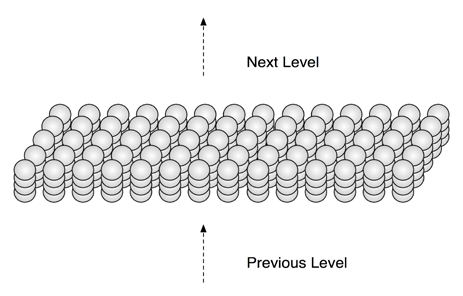
\includegraphics[width=\textwidth]{region_2}
\end{frame}


\begin{frame}[c]{Region - Attributes}
    \begin{itemize}[<+(1)->]
        \item All Regions do basically the same
        \item Based on Biological Regions in the Brain
        \item HTM Regions are similar to Layer 3 of the Neocortex
        \item Can do Inference and Prediction even on complex data
    \end{itemize}
\end{frame}




\subsection{Sparse Distributed Representation}
% \subsection{The Datastructure of the Brain}


\begin{frame}[c,fragile]{Data Saving - Computer Science Solution}
    \Large
    What is \verb|01100101|? \pause Could be either one of:
    % What is ? Could be:
    \begin{itemize}[<+(1)->]
        \item Booleans (\verb|False, True, True, False,|\dots)
        \item Integer (\verb|101|)
        \item Float (\verb|3328.0|)
        \item (Byte-) String (\verb|'e'|)
        \item Pointer to something else
        \item Part of some other Datastructure
    \end{itemize}
\end{frame}


\begin{frame}[c,standout]
    Biological observation: \newline
    We use only part of our brain!
\end{frame}


\begin{frame}[c]{Sparse Distributed Representation - Introduction}
    \Large
    \begin{itemize}[<+(1)->]
        \item Datastructure of the brain
        \item Sparse (around 2\% are active)
        \item Distributed (clusters are somewhat rare)
        \item Inhibitory mechanisms
        \item Neuron states actually have 'meaning'
        \item Combined, they give context as well
        \item Many mechanisms in the brain would not work otherwise
    \end{itemize}
\end{frame}


\begin{frame}[c]{Sparse Distributed Representation - Example}
    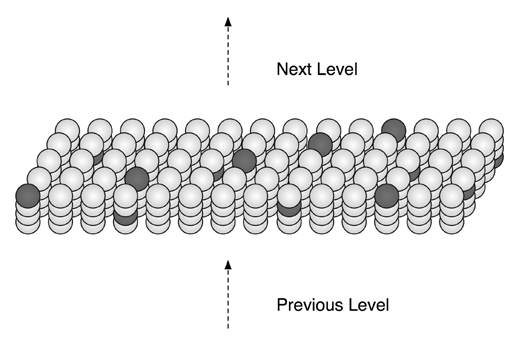
\includegraphics[width=0.95\textwidth]{region_sparse}
\end{frame}


\begin{frame}[c]{Sparse Distributed Representation - Example}
    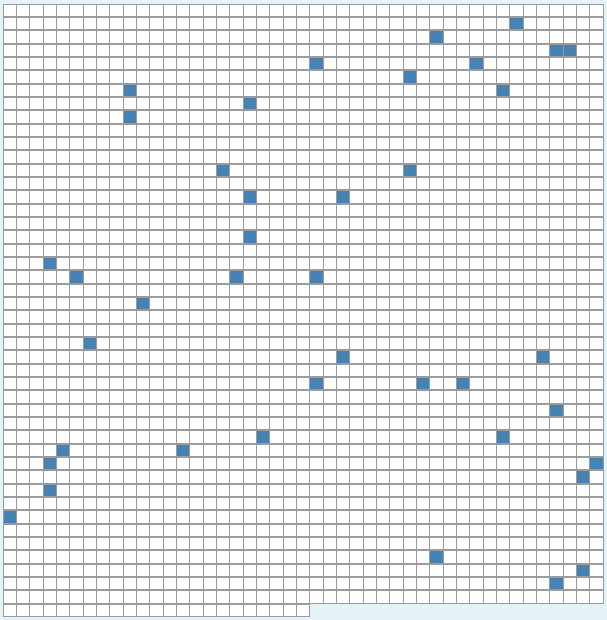
\includegraphics[height=0.9\textheight]{sdr_example}
\end{frame}

% \begin{frame}[c]
    % 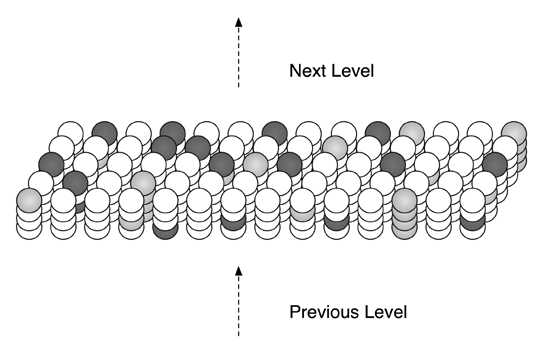
\includegraphics[width=0.9\textwidth]{region_predict}
% \end{frame}


\begin{frame}[c,standout]
    Live Demo!
\end{frame}


\begin{frame}[c]{Sparse Distributed Representation - Live Demos}
    \Large
    \begin{itemize}[<+(1)->]
        \item Ep2/Capacity
        \item Ep2/Matching (Noise resistency)
        \item Ep3/Subsampling
        \item Ep4/Classification
        \item Ep4/Union
        \item Ep5/Scalar Encoding
        \item Ep6/Date Encoding
        \item Ep5/RDSE - Number Encoding
    \end{itemize}
\end{frame}


\begin{frame}[c]{Encoders - Conclusion}
    \begin{itemize}[<+(1)->]
        \item Semantically similar data should result in SDRs with overlapping active bits.
        \item The same input should always produce the same SDR as output.
        \item The output should have the same dimensionality (total number of bits) for all inputs.
        \item The output should have similar sparsity for all inputs and have enough one-bits to handle noise and subsampling.
    \end{itemize}

    \normalsize
    \pause
    Cited from \cite{hawkins2016book}.
\end{frame}



\section{Implications}


% \begin{frame}[c]{Main Brain Task}
%     \pause
%     \Huge
%     What does the brain \textbf{do} \newline all the time?
% 
%     \vfill
% 
%     \pause
%     Predict. \pause Learn.
% \end{frame}
% 
% % intelligence : ability to make models
% % smart : ability to reach your goals
% % wise : picking the right goals
% 
% \begin{frame}[c]{Definition - Intelligence}
%     \Large
%     Intelligence \pause is the ability to create models. \\ \\ \pause
%     Not behaviour. Or anything else.
% \end{frame}
% 
% \begin{frame}[c]{Definition - Understanding}
%     \Large
%     Understanding \pause means to have a precise model about $<$Thing$>$.
% \end{frame}
% 
% \begin{frame}[c]{Definition - Meaning}
%     
% \end{frame}






\section{Open Questions}


\begin{frame}[c]{Open Questions}
    
\end{frame}






% 
\begin{frame}[c]{Relation to Machine Learning}
    \Large
    \pause
    Who has knowledge about Machine Learning? \newline \newline
    \pause
    How similar do you think the Brain really is?
\end{frame}




%%%%%%%%%%%%%%%%%%%%%%%%%%%%%%%%%%%%%%%%%%%%%%%%%%%%%%%%%%%%%%%%%%%%%%%%%%%%%%%%%%%%%%%%%%%%%%%%%%%



%%%%%%%%%%%%%%%%%%%%%%%%%%%%%%%%%%%%%%%%%%%%%%%%%%SOURCES%%%%%%%%%%%%%%%%%%%%%%%%%%%%%%%%%%%%%%%%%%

\section{Sources}
\begin{frame}[c,fragile,allowframebreaks]{Sources}
    \Large
    \vfill
The slides are online: \url{https://github.com/fkarg/things-to-talk-about/blob/master/htm/main.pdf} \vfill
Drop me a mail: fkarg10@gmail.com \vfill \newpage
% \bibliographystyle{plainnat}
\bibliographystyle{ieeetr}
\bibliography{references.bib}
\end{frame}


\appendix
\backupbegin

\begin{frame}[c]{Rust: Code Example}
    \begin{codeboxed}{Code Example 1}
    \inputminted[linenos, fontsize=\normalsize]{Rust}{code/code_ownership.rs}
    \end{codeboxed}
\end{frame}

\begin{frame}[c]{Rust: Code Example}
    \begin{codeboxed}{Output Nr. 1}
        \footnotesize
        \verbatiminput{code/output1.txt}
    \end{codeboxed}
\end{frame}

\begin{frame}[c]{Rust: Code Example}
    \begin{codeboxed}{Code Example 2}
    \inputminted[linenos, fontsize=\normalsize]{Rust}{code/code_ownership2.rs}
    \end{codeboxed}
\end{frame}

\begin{frame}[c]{Rust: Code Example}
    \begin{codeboxed}{Output Nr. 2}
        \footnotesize
        \verbatiminput{code/output2.txt}
    \end{codeboxed}
\end{frame}

\backupend



\end{document}
